% Changing book to article will make the footers match on each page,
% rather than alternate every other.
%
% Note that the article class does not have chapters.
\documentclass[letterpaper,10pt,twoside,twocolumn,openany]{book}

% Use babel or polyglossia to automatically redefine macros for terms
% Armor Class, Level, etc...
% Default output is in English; captions are located in lib/dndstring-captions.sty.
% If no captions exist for a language, English will be used.
%1. To load a language with babel:
%	\usepackage[<lang>]{babel}
%2. To load a language with polyglossia:
%	\usepackage{polyglossia}
%	\setdefaultlanguage{<lang>}
\usepackage[english]{babel}
%usepackage[italian]{babel}
% For further options (multilanguage documents, hypenations, language environments...)
% please refer to babel/polyglossia's documentation.

\usepackage[utf8]{inputenc}
\usepackage{hang}
\usepackage{lipsum}
\usepackage{listings}
\usepackage{graphicx}

\usepackage{dnd}

\lstset{%
  basicstyle=\ttfamily,
  language=[LaTeX]{TeX},
}



% Start document
\begin{document}
	



	\chapter{Agdha Zacharias}
	
	
	\begin{figure}
		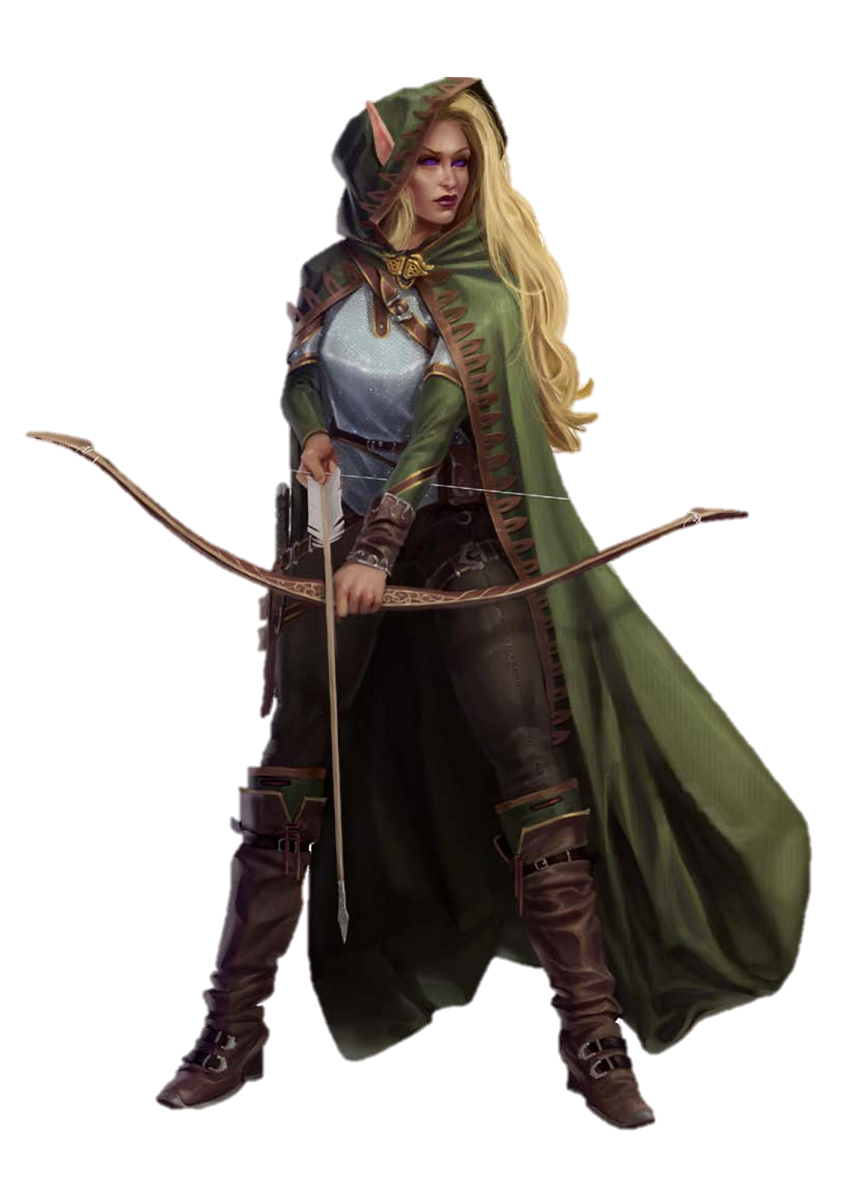
\includegraphics[width=\linewidth]{../elfranger3.png}
		\label{fig:az}
	\end{figure}


	\begin{quotebox}
		Nobody can teach you better than nature, it has been doing so for years.
	\end{quotebox}
	
	
	
	\header{General Information}
	\begin{dndtable}
	
		Race  & Half-Elf \\
		Class  & Ranger \\
		Background  & Outlander \\
		Alignment & Chaotic Neutral \\
		Age & 34 \\
		Origin & Forester \\
		Conclave & Beast Conclave
	\end{dndtable}
	
	\vfill\null

	\section{Background}
		\subsection{Traits}
		Nature raised me, and I have still so much to learn. I want the others to learn the ways of nature as well as they are my friends. I will never pass a chance to teach a lesson about nature. 
		\subsection{Ideal}
		People come and go, their structures as well. They are unimportant in the timeline of the world. What must be protected is the fields and trees, bushes and lakes, rivers and mountains that nature provides. 
		\subsection{Bond}
		One of the few ways to make me an enemy is, … well either kill my whole hometown which has been done before or injure what hurts me most – nature. 
		\subsection{Flaw}
		If you don’t know how to survive out there, no worries I’ll help you. But if you are useless out there you better just stay where you are because bears like a nice snack from time to time. 

	\pagebreak
	
	\section{Story}
	\subsubsection{Early Years}
	The town I was born in was idyllic and quiet. One of the few places in this world where it didn’t matter what race you are and where you come from as long as you were nice to everyone else. My father was an elf, my mother human. I don’t know how the two found each other but I know that my father was thrown out of his clan when they found out. My mother was already pregnant and out of sheer luck they found this little town to live in. My first years were great. My father and I often went on camping trips in the nearby forest. He taught my how to use the longbow and which plants were edible or not. I had a blast back then. Young and naïve I was, I didn’t even know that there’s a war going on on the other side of the forest and that people like me are not welcome in this world. “The empire”, my father used to say, “do not like young half elves like you but don’t worry.”. 
	
	But our idyllic way of living was not for long. One day the soldiers of the empire marched into our city. My father sent me away and after some protesting I gathered my stuff and ran off into the woods, alone. After a week I returned to our town which was now a place of ash and burned corpses. The empire destroyed everything I had. 
	
	\subsubsection{The Woods}
	I started to live in the woods. I was young and even though I went camping a lot I wasn’t prepared. There are beasts in the forest I do not dare speak of. Nature seemed to work against me no matter what I did. I frequently went on for several days without finding any food. Everything changed one day. There were three goblins near my camp. I overheard them say that the ground they stood on was perfect for their clan to reside. They started by making a campfire, which was fine, but soon ignited some torches and burning down foliage, trees and bushes around them. They were about to destroy the forest for their own means! I quickly grabbed my longbow and climbed on a tree. I shot them down with three arrows. I’ve never been angrier at that point and never been this precise. I put out the already burning fire with my bare hands and stayed there to make sure that there are no other goblins approaching.
	
	After this incident the way nature treated me changed. It seemed like nature was starting to respect me after I had saved it from burning down. Even the animals were nicer towards me. I got along well with the smaller ones and they would alert me if there was a predator on the way. I protected the forest and the forest protected me. 
	
	\subsubsection{Mentor}
	The first lesson nature taught me was just a couple of days after the goblin incident. It was night and a little bug crawled on my face. I woke up. This was the first time I felt unwell in the woods. Something wasn’t quite right. I snuck out of my campsite and wandered around as quietly as I could. But my feet seemed to be louder than usual on the forest floor. I heard each leaf I stood on. Soon I realized what was wrong. The forest was dead silent. Not a single bug or bird was to be heard. I stood still in my tracks and started to listen more carefully, after I managed to ignore my own breath I heard an eerie sound. Like someone mimics wind with their own mouth far in the distance. I jumped behind the closest tree and sat down. Trying to be as silent as possible. I observed some moon flowers, which bloom at night, close their leaves and face downward. This was highly unusual. After a few more minutes I saw what they were turning against from. A dark creature, much like a shadow, was passing through the woods. About 500ft away from me. I held my breath trying to make no sound at all. When the flowers were not facing the creature, why should I? The shadow creature went further away. The weird thing was, it passed through the trees as if they weren’t there. I sat by that tree until the morning sun arrived and the flowers around me started blooming again. That was the night I learned that nature knows so much more than we do. 
	
	\subsubsection{Animals}
	The woods were very lonely at times. I sometimes feared that I'll soon forget how to speak. That's probably why I bond with animals so much. The smaller ones often slept near me and played with me during my younger years. If one was hurt they'd lead me to it and I'd try my best to get it back on track. Sometimes I feel I could speak with them, read their minds. I mostly know exactly what these creatures want. I adapted to them. But most animals in the woods have a short life span and it broke my heart every time I lost a little friend. 
	
	\subsubsection{Challenges}
	After about 15 years in the woods I decided it was time to go out and meet some other beings than animals. I've seen many towns near the edge of the forest and went to the one that I had deemed most safe. It felt really weird being around people but my fear that I forgot how to speak soon proved itself wrong. I got along with the people there. Problem was that I had no money and couldn't just sit with them and have a drink. Some human must have realized this and offered me a little "challenge" as he called it. He bet me that I could not shoot a specific apple off the nearest tree. I took that challenge and asked him which apple he wants. As he was pointing to it I quickly drew my longbow and shot away. The apple fell on the ground - in it my arrow. I got to keep the apple and he gave me some metallic coins. He told me that would be enough to have a drink at the bar with him. He introduced himself as Arno.  
	
	In the bar we talked about our past lives. The human had a rather boring life but I learned that he was quite rich. I didn't really care for human wealth but after a while of pretending to, he offered me a job at his mansion. He has pissed someone off and wanted me to protect the house while he sleeps until the danger is over.
	 
	I took the job. He offered me a guest room to sleep in during the days but it was really uncomfortable and I felt trapped in that little room. After that I slept outside. 
	
	Arno told me more about this other guy. Apperiantely it was a goblin that was living in a cave Arno owns. Arno tried to throw the guy out so he could use the cave as secure storage but the goblin, which goes by the name Blacks, would not move. So Arono flooded the cave out of despair. Blacks got out but screamed murder. Arno later learned that Blacks was a hitman and was now after him. 
	Many nights went by without something happening. But one night Blacks finally showed up. He must have learned my walking patterns and got to the mansion unnoticed. I only realized he's there because he had to break the door and I happened to heard that. I chased him into the mansion and we fought. It was a hard fight but in the end I was able to stab Blacks in the heart with my shortsword. 
	
	Arno payed me a lot of coins and I went on, switching between living in the woods and doing small jobs for strangers. 
	
	\subsubsection{Striking back}
	One day while making my rounds in the woods a little squirrel approached me. It was furious, would climb up and down my cape and I felt it wanted me to follow it and so I did. The squirrel ran through the forest, then through fields and through rivers. It was hard to keep up, but I felt it was important. Soon I saw black smoke rising from a little town in the distance. I saw soldiers much like the ones that invaded my little home town. Suddenly I was even more furious than the squirrel and overtook it. In the city, which I later got to know as “Goldfield” was a huge fight going on. Empire against the common people. It wasn’t hard to decide which site to root for. I shot some arrows from the distance, it may hit one or two soldiers, but they were stronger than the goblins back then. In the middle of the city there was a group of people from different races together fighting. I really liked the view of them uniting against the greater force and joined them in the fight. There was a gnome, another half-elf and even a tiefling. 
	
	After a lot of fighting and many causalities on our side, victory was ours. The last soldiers of the empire were either dead or fleeing the city. The other adventurers were as happy as I was. Later, in the middle of celebration, I noticed the little squirrel on the gnome’s shoulders. 
	
	

	\chapter{Fuldrock Harvan}
% Male Hill Dwarf, Chaotic Good, Philosopher
% Trait: Talks slowly to dumb people
% ideals: self improvement, study
% Bonds: Librarys, university, scriptorium, monastery
% Flaws: Speaks without thinking, insulting others
% Astronomer
% Takes trophies from all kills
% Worships God of Pleasure and War Hittunna
% Secret: is beyond rich
% Mother Mara, Father Draksesh Brother Devrock, Son Merlack
	\begin{figure}
		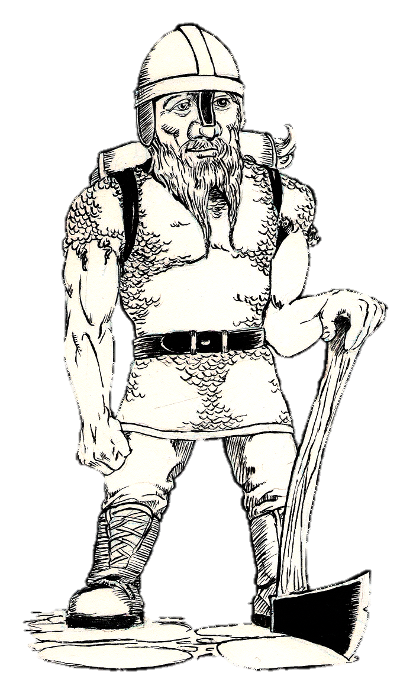
\includegraphics[width=\linewidth]{../fuldrock.png}
		\label{fig:az}
	\end{figure}
	
	
	\begin{quotebox}
		The stars show us the way, but you wouldn't understand. 
	\end{quotebox}
	
	
	
	\header{General Information}
	\begin{dndtable}
		
		Race  & Hill Dwarf \\
		Class  & Socerer \\
		Alignment & Chaotic Good \\
		Age & 288 \\
		Size & Medium 
	\end{dndtable}

	
	\vfill\null

	\section{Background}
		\subsection{Traits}
		I talk really slowly to people i perceive as dumber than me. And I have rarely met someone on my level.
		
		Also if I kill someone, I keep a little trophy reminding me of my victory. 
		\subsection{Ideal}
		We need to learn something new every day. Knowledge is more powerful than any weapon. 
		\subsection{Bond}
		Knowledge must be preserved. There is nothing more meaningful in the world as books and universities that teach. Thus my favourite place is in a quiet library sitting on a leather chair and learning something new. 
		\subsection{Flaw}
		I just say what I think and I don't care if I'm too harsh. 
		\subsection{Secret}
		I am staggering rich, you can't believe how much money I have. But I won't tell you anyway. 
	\pagebreak

	\section{Story}
		\subsubsection{Early Years}
		My mother Mara always says that the stars were shining bright the night I was born. She says she knew even before I let out my first scream that I will be something special. And she was right. I could read before my five year older brother Devrock and gasped the basic physical principles before attending school. Although I don't understand why not everyone is capable of this, because it isn't that hard. 
		
		My brother and I went to a prestige school. How much my parents paid to get him into this elite school, I don't know. But with a little help of me he got through. He helped me get some friends in return. It was hard for me to find other pupils that were on my level of intelligence. But my brother frightened some of them so much that they talked to me regularly. That was aright with me. After school finished I went on to university and Devrock went back to our parents to help them with their business. 
		
		University was finally my time to shine. My knowledge was looked up on and the professors liked me and talked with me on a level I didn't have to dumb myself down. I chose astronomy as my major. The only major that challenged me really.
		
		\subsubsection{Family} 
		Our father Drakesh owns a business where he engineers and builds new mining gear for the mines. He also plans the most efficient ways to get to the precious ores. Drakesh is a very smart man and he found the perfect mate, my mother Mara. Mara used to work at the university before joining my father in the business. She is a professor in sorcery and arts. She completes Drakesh with her beautiful and creative way of thinking. My brother Devrock is everything we are not. He is a hard working guy but there's not much in his head. But he makes that up by being the most honest and loyal dwarf you'll ever meet. The Harvans stick together no matter what. 
		
		\subsubsection{Leaving Home}
		It is tradition in our family that the males leave the home and wander around the world when they turn 100. Even if they got family at home they need to go for at least twenty years to experience the live outside our wealth. I was really excited for it. My brother left five years ago and has sent letters about how nice he has it and how he found some jobs to do and found new friends. I was mostly looking forward to travel to other universities and read books our library didn't have. I wanted to learn new things. So on my 100th birthday I kissed my mother goodbye, bowed to my father and left. 
		
		The first thing I did was not really a smart move on my side. Probably the first dumb thing I've done in my life then. On the first day I just went a town over. I booked a room in the tavern there and went down to have a drink. Next thing I knew was that I was laying behind a bush, it was daylight and my head hurt. Everything I took with me was gone. I was robbed. Luckily I only took some money down to have a drink and the other part I hid in the room I booked. The room was open and it looked like someone went through everything but they didn't get to my secret stash of gold coins. But that didn't really matter to me then, all the books I packed were gone. I nearly started to cry but I was a grown dwarf now and I shouldn't be crying. I was too ashamed to head back home and went further south. In hindsight this was a great lesson even thought it could have been taught less hurtful. 
		
		\subsubsection{Love}
		All my life up to this point I just had much older professors or frightened kids as friends. I had no one who I really connected with.  One day while I was fighting off some twig blights for some guy that wanted to build his house in a middle of the forest I saw her from a distance. Madeline. She was a beautiful dwarf wandering the woods all by herself. Her blonde hair looked unusual but somewhat also just plain perfect on her. I quickly chopped off the head of the blight and took a little twig from it and put it in my pocket. I ran up to the beautiful woman and started to introduce myself. She seemed delighted by my appearance and we started talking. I learned that she was in the woods trying to find some plants for her potions. She was a professor at the nearest university and I instantly knew that this was the girl I will love the rest of my live. I moved in with her and after my twenty year period of wandering the world I took her back to meet my family. 
		
		\subsubsection{Child}
		Madeline was soon pregnant and bore me a wonderful son, Merdlack. He got his mothers hair and my eyes. I loved my son and taught him everything I knew. He was so bright and learned fast. He went to the same schools as I and chose sorcery as his major. He seemed to come after his mother and grandmother. Both were so proud. Devrock taught him basic fighting skills and he was so talented. After my parents death I took over Fathers business. It wasn't exactly my field but with the help of Madeline I could keep up the sales and the innovation. 
		
		On Merdlack's 100th birthday he set out to see the world. With his wish to find a perfect match like I had. We waved goodbye and were so proud of him.
		
		We haven't received a single letter from him. We thought that he just went further than usual.
		
		After twenty years he hasn't returned home. We thought he just forgot the time. 
		
		After twenty five years my wife became sick out of sadness that Merdlock hasn't come home.
		My wife died after thirty years of Merdlock absence. 
		
		A day after that I set out into the world once again to find out what has happened to my son.  

	
	\vfill\null

	
	

		
		
		

	
% End document
\end{document}
